\documentclass{standalone}

\usepackage{amsmath}
\usepackage{tikz}
\usetikzlibrary{arrows.meta, positioning, calc, }

\begin{document}

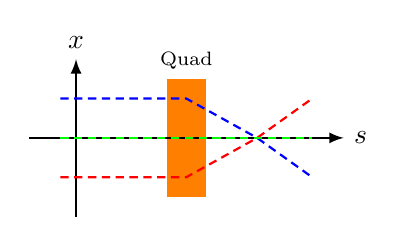
\begin{tikzpicture}[>=latex]
    \coordinate (O) at (0, 0);

    \pgfmathsetmacro{\sini}{1.6}  
    \pgfmathsetmacro{\dy}{0.5}  
    \coordinate (Op) at (0, \dy);
    \coordinate (Om) at (0, -\dy);

    \coordinate (Ep) at (\sini, -\dy);
    \coordinate (Em) at (\sini, \dy);

    \coordinate (F) at (0.9, 0);

    \pgfmathsetmacro{\qlarg}{0.5}   
    \pgfmathsetmacro{\qalt}{1.5}

    \path[fill=orange, draw=none] ($(O)+(\qlarg/2,\qalt/2)$) rectangle ($(O)-(\qlarg/2,\qalt/2)$);
    \node[above] at ($(O)+(0,\qalt/2)$) {\scriptsize Quad};

    \draw[thick, ->] (-2, 0) -- (2, 0) node[right] {$s$};
    \draw[thick, ->] (-\sini+0.2, -1) -- (-\sini+0.2, 1) node[above] {$x$};

    \draw[thick, densely dashed, blue] (-\sini, \dy) -- (Op) -- (F) -- (Ep);
    \draw[thick, densely dashed, red] (-\sini, -\dy) -- (Om) -- (F) -- (Em);
    \draw[thick, densely dashed, green] (-\sini, 0) -- (\sini, 0);

    % \draw[line width=0.7pt, black, stealth-, densely dotted] ($(F) - (0, 0.7)$) -- (F);
    % \node[below] at ($(F) - (0, 0.7)$) {\small $\frac{1}{KL}$};

\end{tikzpicture}


\end{document}